\section{Design and Implementation}
\label{sec:implement}

\NM{} is designed as a replacement memory allocator. It intercepts all memory allocation/deallocation invocations via the preloading mechanism, and redirects them to \NM{}'s implementation. Therefore, there is no need to change the source code of applications, and there is no need to use a custom OS or hardware. In the following, we first discuss \NM{}'s overall design, and then discuss multiple components that separate it from existing allocators.

\subsection{Basic Heap Layout}
\label{sec:overview}

\begin{figure}[!ht]
\begin{center}
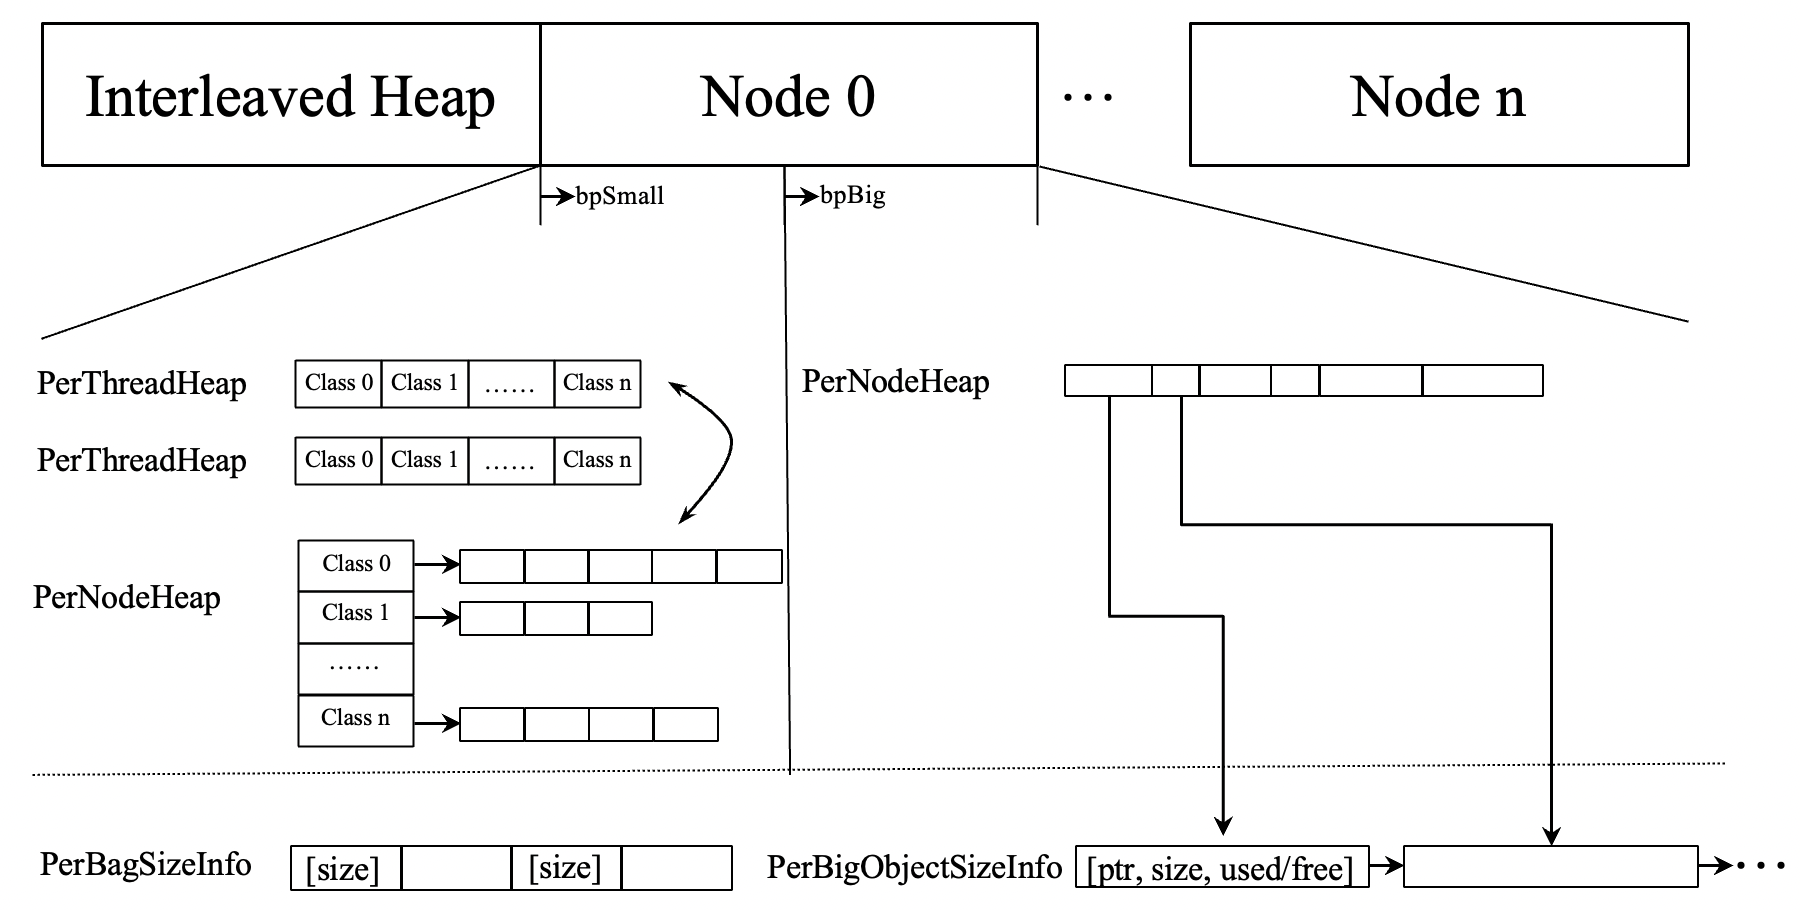
\includegraphics[width=0.45\textwidth]{SC2022/figure/numalloc-overview.png}
%\includegraphics{figure/overview2}
\end{center}
%\vspace{-0.1in}
\caption{Overview of \NA{}'s heap layout.
\label{fig:overview}}
%\vspace{-0.1in}
\end{figure}

% \todo{We should balance what to talk about in the overview, it's a little bit long and something has repeatedly described in the following}

%As discussed in Section~\ref{sec:intro}, \NM{} designs a origin-computable mechanism that could quickly check the origin of every object upon deallocation. In order to support this, 
\NM{}'s heap layout is designed as  Fig.~\ref{fig:overview}. Initially, \NM{} requests a large and continuous block of memory from the underlying OS, and then divides it evenly into multiple regions based on the number of hardware nodes. Each region is bound to a different physical node via \texttt{mbind} system call. 
%\NM{} can support the customized binding from users. If not, it typically  
In particular, the first region is bound to the first node, the second one is bound to the second node, and so on. This design enables us to compute the physical node quickly from a memory address: we could compute the index of the physical node by dividing the heap offset by the region size. 
%This layout is different from existing allocators, based on our knowledge. 
% \todo{Numalloc's reviewer said TCMalloc also use the same mechanism. I check the code and it's true that TCMalloc use the memory tag for numa partition id}

%\NM{} borrows some of these existing mechanisms. First, it uses different mechanisms to manage small and big objects. Second, small objects are also managed by size classes using the BiBOP-style. Third, similar to existing work, such as Linux and TCMalloc~\cite{tcmalloc}, \NA{} utilizes different freelists to track freed objects, and uses the first word of freed objects to link different objects. But the difference of \NM{} is further described in Section~\ref{sec:implement}.

From Fig.~\ref{fig:overview}, we see that each node's memory region will be further divided into two sub-regions, one for small objects, and the other one for big objects. The \texttt{bpSmall} pointer is utilized to track never-allocated memory for small objects, and big ones are tracked with \texttt{bpBig} pointer. Similar to existing allocators, \NM{} manages small and big objects differently. In \NM{}'s design, small objects are those with a size less than 512K, which are organized by size classes and each request will be satisfied from a particular size class. \NA{} utilizes fine-grained size classes for small objects, such as 16 bytes apart for objects less than 128 bytes, and 32 bytes apart for objects between 128 bytes and 256 bytes, then power-of-2 sizes afterward. For small objects, \NM{} utilizes the well-known ``\textbf{Bi}g-\textbf{B}ag-\textbf{o}f-\textbf{P}ages'' (BiBOP) style that all objects in the same bag (32 KB by default) will have the same size class. 
Big object allocation will be satisfied in a sequential manner and their sizes are aligned to the size of one bag (32 KB).

To support the NUMA architecture, a per-node heap (PerNodeHeap in Fig.~\ref{fig:overview}) is proposed that has one freelist for each size class and one common freelist for all big objects from the current node. 
%We will talk about the relationship between per-thread freelist and per-node freelist in Section~\ref{sec:origin}. 
%For small objects, freed objects of the same size class will be tracked with a freelist.
In order to reduce the contention, \NM{} adopts a per-thread heap (PerThreadHeap in Fig.~\ref{fig:overview}) that maintains a freelist for each size class, which requires no lock protection since each thread has its own per-thread heap. However, this may introduce memory blowup~\cite{Hoard} that freed objects of a per-thread heap cannot be utilized for future allocations from other threads, which will be addressed in Section~\ref{sec:others}. 
\NM{} tracks the small objects' size information in a separate area called PerBagSizeInfo, while the big objects utilize a linked list called PerBigObjectSizeInfo to store the size and availability information, which allows coalescing multiple continuous big objects into a bigger object upon deallocations.

% \NM{} tracks the size information and availability information in a separate area:  ``PerBagSizeInfo'' of Figure~\ref{fig:overview} is used for tracking the size of each size class for small objects.

%(shown as ``PerMBInfo'' of Figure~\ref{fig:overview}): it tracks the size of each size class for small objects, and the size of the big object (aligned to 1 MB) for big objects. This data structure also includes the used/free information for big objects, which allows coalescing multiple continuous big objects into a bigger object upon deallocations. To save space, \NM{} utilizes the lowest significant bit of ``PerMBInfo'' to encode the availability information.

Overall, \NM{} includes a layout to quickly compute the physical node (with the memory binding) and a per-node heap to support node-aware allocations. This design allows it to perform origin-aware memory management efficiently, as discussed in the next section. 

%mechanisms to re and one per-node freelist for each node to track big objects. \NM{} also maintains per-node freelists to track small objects based on size classes. These freelists are singly linked lists, which uses the first word of every freed object as pointers.  Small freed objects may be migrated between per-thread freelists and per-node freelists, as further described in Section~\ref{sec: others}. 
\subsection{Binding-Based Memory Management} 
\label{sec:balance}
As described in Section~\ref{sec:intro}, thread migration will cause multiple performance issues for the NUMA architecture. Therefore, \NM{} binds each thread to a node specifically in order to avoid thread migration across different nodes. Currently \NM{} currently supports two types of binding, \textbf{node-interleaved binding} and \textbf{node-saturate binding}, where users could provide their customized binding as well. Node-interleaved binding binds continuous threads to different nodes in an interleaved way so that every node will have a similar number of threads. That is, the first thread will be bound to the node that it is scheduled to run by the OS, and the second thread will be bound to its next node, and so on. Instead, the node-saturate binding will bind sufficient threads to a node first before binding to a different node. For node-saturate binding, threads to be assigned will be the same as the number of hardware cores.  

Note that \NM{} only binds a thread to a node, instead of a core, which still allows the scheduling initiated by the OS. To perform the binding correctly, \NM{} obtains the hardware topology in the initialization phase via the \texttt{numa\_node\_to\_cpus} API, which tells the relationship between each CPU core and each memory node. Then it intercepts all thread creations in order to bind a newly-created thread to a specific node.
%In the future, we plan to support more user-controlled binding. 

%\subsection{Selective Huge Pages} 
%\label{sec:hugepage}

%Based on the existing study~\cite{hugepages}, huge pages can reduce Translation Look-aside Buffer (TLB) misses, since the same size of TLB entries will cover a larger space of memory. However, existing transparent huge page support is not good for the performance~\cite{Gaud:2014:LPM:2643634.2643659, DBLP:conf/asplos/PanwarBG19}, due to hot page effect, page-level false sharing, and increased memory footprint~\cite{DBLP:conf/asplos/MaasAIJMR20}.
 
%\NM{} proposes explicit huge pages to avoid these issues that could always benefit the performance based on our evaluation in Section~\ref{sec:hugepage}. The basic idea of \NM{} is to carefully choose which objects that should be allocated from huge pages: first, shared objects should not be allocated from huge pages, which may introduce page-level false sharing that multiple threads are accessing the same huge page. This will cause unnecessary load imbalance due to concurrent accesses, and remote accesses. Second, if we only utilize partial memory in the same huge pages, then we may waste the remaining memory on the same page. This problem will become more serious for \NM{}'s design, since it is using a big bag (1MB) to hold objects of the same size. 

%If huge pages are only utilized for private objects for threads running on the node, then there is no hot page effect and page-level false sharing. Also, if huge pages are only utilized for big objects that are larger than the page size, then there is no need to worry about unnecessary memory consumption. 
%Based on these observations,  \NM{} only employs huge pages for large objects, with a size larger than 512KB. This design will reduce unnecessary memory waste that only partial pages are actually allocated. Also, \NM{} only employs huge pages for small objects that are predicted to be allocated frequently. For the latter one, \NM{} employs the history information to predict, and only uses huge pages for a size class that has used at least one bag before. Based on our evaluation in Section~\ref{sec:hugepage}, this design balances the performance and memory consumption, which always benefiting the performance. 

%In addition to large objects that has the size larger than the size of a huge page, huge pages are only utilized for small objects that are predicted to be used a lot.  \NA{} employs the history of memory allocation to predict this. 
%Each per-node heap is further divided into two parts as illustrated in Figure~\ref{fig:overview}: small objects will be allocated from the first half and will be allocated using small pages, while big objects will be allocated from the second half with huge pages (2MB). When a big object (with the huge page) is utilized for small objects, only frequently-allocated small objects can utilize such an object. We believe that our design balances the performance and memory consumption.   


\subsection{Threads-shared Incremental Allocation}
\label{sec:hugepages}
When Transparent Huge Page (THP) is enabled, the OS will prefer to allocate huge pages if a program touches a continuous memory region with the size larger than a huge page (e.g., 2MB). Since \NM{} allocates a large region initially (as shown in Fig.~\ref{fig:overview}), huge pages will be employed by the OS correspondingly. However, it is important to reduce memory fragmentation, as one allocation from a memory block will be assigned to a huge page. \NM{} makes multiple threads (from the same node) share the same memory block, instead of having a separate super-block for each thread as Scalloc~\cite{Scalloc}. That is, when a thread is running out of memory, it obtains only multiple objects at a time (currently 32K) from the corresponding memory block, instead of getting few megabytes for each per-thread heap. To get rid of the unnecessary memory overhead on metadata, such as ``PerBagSizeInfo'' used internally by \NM{}, we leverage \texttt{madvise} system call to make it allocated from normal pages. These are the basic reasons that \NM{} has much less memory consumption than Scalloc, as evaluated in Section~\ref{sec:memory}. 

\subsection{Other Mechanisms}
\label{sec:others}

\NM{} also implements the following mechanisms in order to improve the performance.

\subsubsection{Origin-Aware Memory Management} 
\label{sec:origin}

%\todo{In Section III-B, you talk about satisfying allocations from the "un-allocated region" as the last step. Is this memory that is not part of the interleaved heap? It would help to be more clear about what this is. }

As described in Section~\ref{sec:overview}, \NM{} includes an origin-computable design that could quickly determine the origin of each object via the computation. 
%On top of it, we further discuss other aspects of \NM{}'s origin-based memory management as follows.
On top of it, \NM{} proposes an origin-aware deallocation that will always return a freed object to a freelist with the same origin. In particular, if a freed object is originated from a different node, it is returned to its original node's  freelist. Otherwise, a small object is returned back to the thread's freelist and a big object is returned back to the current node's freelist. Comparing to node-based freelist, there is no need to acquire a lock when operating on the per-thread freelist. Different from all existing work, \NM{} may return a freed object into the per-thread list or its original node's freelist, instead of simply putting into the per-thread list. That is, \NM{} considers the originality of objects for deallocations. 

\NM{} always ensures node-local memory allocations. For small objects, it follows this order: (1) The per-thread's freelist will be checked first, since there is no need to acquire any lock and objects may be still hit in the cache (as they are just accessed by the thread). (2) If the per-thread freelist does not have available objects, \NM{} tries to allocate from the current node's freelist. As mentioned above, a node's freelist holds objects originated from this node. (3) If the previous two steps fail,  we will allocate the memory from the current node's un-allocated region, as shown by \textit{bpSmall} in Fig.~\ref{fig:overview}. 
%Since the region is bound to the current node, and objects in the per-thread freelist and the per-node freelist are always originated from the current node, 
%\NM{} ensures local allocations for small objects. 
For big objects, allocation will be satisfied from per-node freelists or un-allocated region (pointed by bpBig pointer in Fig.~\ref{fig:overview}) of the current node, indicating local allocations for big objects. 

\subsubsection{Interleaved Heap} 
\NA{} proposes an interleaved heap that is inspired by existing profilers\cite{XuNuma, MemProf}: \textit{many NUMA performances issues are related to shared objects allocated in the main thread}. Due to the default first-touch policy~\cite{lameter2013numa, diener2015locality}, objects allocated and touched by the main thread are typically allocated in the node that the main thread is running on. However, these objects can be passed to multiple child threads and be accessed by these threads concurrently so that this node's memory controller becomes the performance bottleneck. 

To reduce this issue, \NA{} reserves a range of memory for such objects, called ``Interleaved Heap'' as shown in Fig.~\ref{fig:overview}. \NA{} utilizes the \texttt{mbind} system call to specify that physical pages of this heap will be allocated from all nodes interleavedly. With this design, when these objects are passed to child threads, these threads may access objects that are allocated from multiple nodes, reducing interconnect congestion and load imbalance of a single node. 

As we evaluated in Section~\ref{sec:interleavedheap}, the interleaved heap is beneficial to the performance for some applications. However, it may degrade the performance, especially when an application spends a lot of time in its serial phase. With the default first-touch policy, all accesses in the first serial phase will be local accesses, but the interleaved heap will turn some local accesses to remote ones. Therefore, the interleaved heap is provided as an option that can be enabled whenever necessary. 


\subsubsection{Efficient Object Movement} 
\label{sec:movement}
%It is important to reduce memory blowup that freed objects by one thread cannot be utilized by other threads~\cite{Hoard}. 
\NM{} requires to move freed objects between per-thread and per-node freelists frequently. An efficient mechanism is required to support frequent movement. However, existing allocators, such as TCMalloc~\cite{tcmalloc}, traverse the freelist to collect a specified number of objects, and then moves all of them at a time, which unfortunately have the following issues:  traversing a freed object will bring some data to the cache unnecessarily, when these objects are moved to other threads later; it will move recently-freed objects (and hot in cache), which is not good for the performance; the traverse of some shared lists may introduce significant lock contention. 


\begin{figure}[!h]
\centering
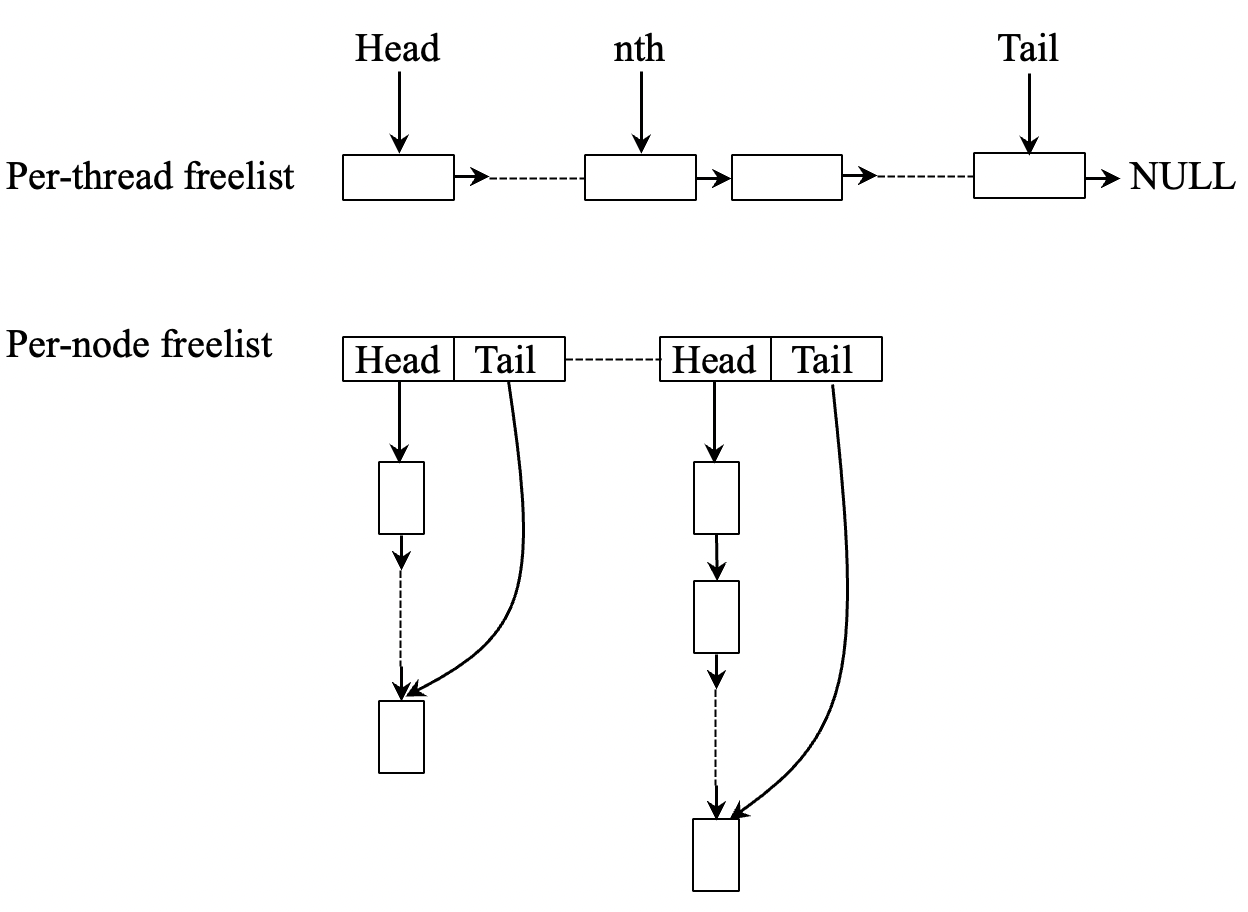
\includegraphics[width=3in]{SC2022/figure/efficient-movement.png}
%\vspace{-0.1in}
\caption{Per-thread freelist and per-node freelist design to achieve efficient object movement.\label{fig:perthreadlist}}
%\vspace{-0.1in}
\end{figure}


\NM{} proposes an efficient mechanism with the following data structures. First, each per-thread freelist maintains two pointers that point to the least recently used objects, shown as the \texttt{Tail} pointer and the $nth$ pointer (counted from the tail) in the upper part of  Fig.~\ref{fig:perthreadlist}. 
This structure avoids the traverse of freelist during the movement, and allows the movement of the least recently used objects (between $(n+1)th$ and $Tail$) to the per-node freelist. After the movement, the \texttt{Tail} pointer will be set to the original $nth$ object. 
Second, \NM{} also proposes a circular array shown in the bottom part of Fig.~\ref{fig:perthreadlist} that helps move objects from per-node (shared) freelist to per-thread freelist. 
%As mentioned above, the per-node freelist could easily become the performance bottleneck, since multiple threads may compete for it concurrently. To address this issue, 
Each per-node freelist actually consists of many sub-lists, where a \texttt{Head} pointer and a \texttt{Tail} pointer point to the header and the tail of each sub-list. When a thread is moving multiple objects from the per-node freelist, it could move all objects in a sub-list (pointed by a pair of \texttt{Head} and \texttt{Tail} pointer) at a time. Therefore, there is no need to traverse the whole list to obtain these objects for the movement, which could reduce the contention. 


%Note that this array does not increase the overhead of putting objects. If a thread puts a freed object to this array, the object can be placed into the current sub-list in a constant time. Similarly, a freelist could be appended to the current sub-list in a constant time. 



\begin{comment}
\begin{wrapfigure}{r}{0.6\textwidth}
\centering
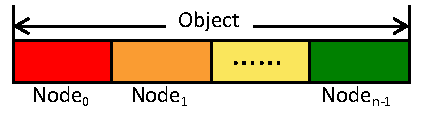
\includegraphics[width=3in]{figure/blockwise}
\vspace{-0.1in}
\caption{Block-wise Memory Allocation\label{fig:blockwise}}
\vspace{-0.1in}
\end{wrapfigure}
\end{comment}

%In theory, private objects of the first thread should not be allocated from the interleaved heap, since that will create remote accesses unnecessarily. Initially, each allocation is treated as a shared one and is allocated from the interleaved heap. Whenever a new thread is created, the allocations are regarded as private ones. Programmers can control whether they want the interleaved support or not based on their applications.


%\NM{} utilizes a simple heuristics to differentiate shared objects from private objects based on allocation callsites: each allocation callsite is treated as a shared one initially, and is allocated from the interleaved heap; Whenever an object is deallocated before creating children threads, indicating such an object is a private one for the main thread, all objects from the corresponding callsite are considered to be private ones, and they are only allocated from the per-node heap afterward. With this heuristics , there is no need to change programs explicitly, although it is more efficient if programmers could provide such information. 

% As mentioned above, \NM{} monitors the  allocation/deallocation pattern of the main thread to identify the share-ability of each callsite. 
%If an allocation callsite is found to be private, then all allocations from this callsite should not allocate from the interleaved heap, but from the normal heap. 
% A challenge is to obtain and compare the callsite of each allocation so that we could determine the heap based on the share-ability. In fact, this may introduce high overhead for applications with large amount of allocations, if using the \texttt{backtrace}~\cite{DBLP:conf/icse/SumnerZWZ10, DBLP:conf/cgo/ZengR0AJ014}. For the performance reason, \NA{} utilizes the sum of the stack position and the return address of the allocation invocation to identify a callsite, called ``\textit{callsite key}''. This combination is able to differentiate callsites correctly if an application does not have allocation wrappers, since the stack position can be utilized to identify the function in the stack and the return address tells the invocation placement inside the same function. If a callsite is misidentified, it will not cause any correctness issue, but with some performance penalties/losses. \NA{} utilizes a hash table to track the status of every callsite. 
 % which is fortunately not very expensive given the limited amount of different callsites. 
 
%Note that the interleaved heap cannot be achieved by using existing NUMA utilities like \texttt{numactl}. Although \texttt{numactl} could also specify memory allocations to be interleaved. However, \texttt{numactl} could only set the policy for a whole application. Instead, \NM{} only utilizes the interleaved heap for shared objects that are allocated in the main thread, not for all objects. 

%\todo{I remove the "Node-Local Metadata" part}

%\subsubsection{Node-Local Metadata} 
%To further reduce remote accesses, \NM{} ensures that all of the metadata is always allocated in the same node. Such metadata includes the metadata for managing per-node lists, per-thread lists, and size class information. Note that ensuring the node-local metadata for per-thread information is only possible when each thread is bound, which is the reason why \NM{} develops the ``binding-based'' approach. Therefore, \NM{} is able to guarantee that all metadata are always allocated in the same node, based on its thread binding as described in Section~\ref{sec:balance}.  
%Such metadata includes per-node and per-thread freelists for different size classes, and freelists for big objects. Similarly, \NM{} utilizes the \texttt{mbind} system call to bind the memory to a specific node.  


%Based on our evaluation, this mechanism reduces most of the memory consumption, with the transparent huge page support by default.  

 %every thread has its own freelists for each size class so that there is no need to acquire the lock when an allocation can be satisfied from its per-thread heap, similar to TCMalloc. That is, two threads will not share the same per-thread heap. However, some applications may create new threads after some threads have exited. \NM{} re-utilizes the memory for these exited threads. Basically, \NM{} intercepts thread joins and cancels so that it can assign heaps of exited threads for newly-created threads, and re-utilize their heaps correspondingly.  


%\paragraph{Transparent Huge Page Support:} During the development, we noticed that excessive memory consumption can be imposed when the OS enables transparent huge pages by default. In order to reduce memory consumption, \NM{} makes multiple threads share the same bag (for the same size class), instead of having a separate bag for each thread. If each thread is running out of the memory, it obtains multiple objects at a time from the corresponding bag. Currently, if a class size is less than one page, then we will at most get objects with the total size of one normal page. Otherwise, it will get 4 objects (with the size less than 64 KB) or 2 objects afterward. Based on our evaluation, this mechanism actually reduces the memory consumption for multiple times for a machine with 128 cores and 8 nodes, with the transparent huge page support by default.  

%\paragraph{Cache Warmup} \NM{} also borrows the cache warmup mechanism of TCMalloc~\cite{tcmalloc}: it will insert all objects in a page into the freelists, if there is no objects in the per-thread freelist. We believe that inserting multiple objects into the freelist will benefit data prefetches, since the insertion is a simple and predictable pattern. With this mechanism, \texttt{raytrace} improves the performance by 10\%. However, this is the only application that we observed such performance improvement. There is no impact on other applications. 

%TCMalloc utilizes a \texttt{mmap} system call to obtain multiple pages (depending on the class size) from the OS each time, when it is running out of the memory for one size class. For such a memory block, TCMalloc inserts all objects of this block into its central freelist at one time. Since TCMalloc utilizes the first word of each object as the pointer for the freelist, this mechanism warms up the cache by referencing the first word of each object during the insertion. According to our observation, this warmup mechanism improves the performance of one application (\texttt{raytrace}) by 10\%. Based on our understanding, the performance improvement is caused by data prefetches, since inserting objects to the freelist has a simple and predictable pattern. \NM{} employs a similar mechanism for small objects with the size less than 256 bytes, and adds all objects inside a page to the per-thread freelist. 

%we propose the combination of per-node heap and per-thread cache. In order to reduce the contention, \NM{} will obtain multiple objects at a time from the per-node heap. 

 
%https://queue.acm.org/detail.cfm?id=2852078

